\section{Acceleration Data Structures}

There are three general techniques to speed up ray tracing. These are fewer intersection computations, fewer rays and generalized rays. We will focus on the first one, trying to calculate fewer intersections. \medskip

Ray-surface intersection is at the core of every ray tracing algorithm, the brute force approach computes the intersection of every ray with every primitive. That are many unnecessary ray-surface intersection tests. \medskip

Before we look at the actual acceleration data structures, we need to define the \textbf{axis aligned bounding box} (AABB). This bounding box aligned with the three axis of our coordinate system and can be defined by two points $min$ and $max$. We can then calculate if a ray intersects a bounding box by the following calculations:
\begin{center}
	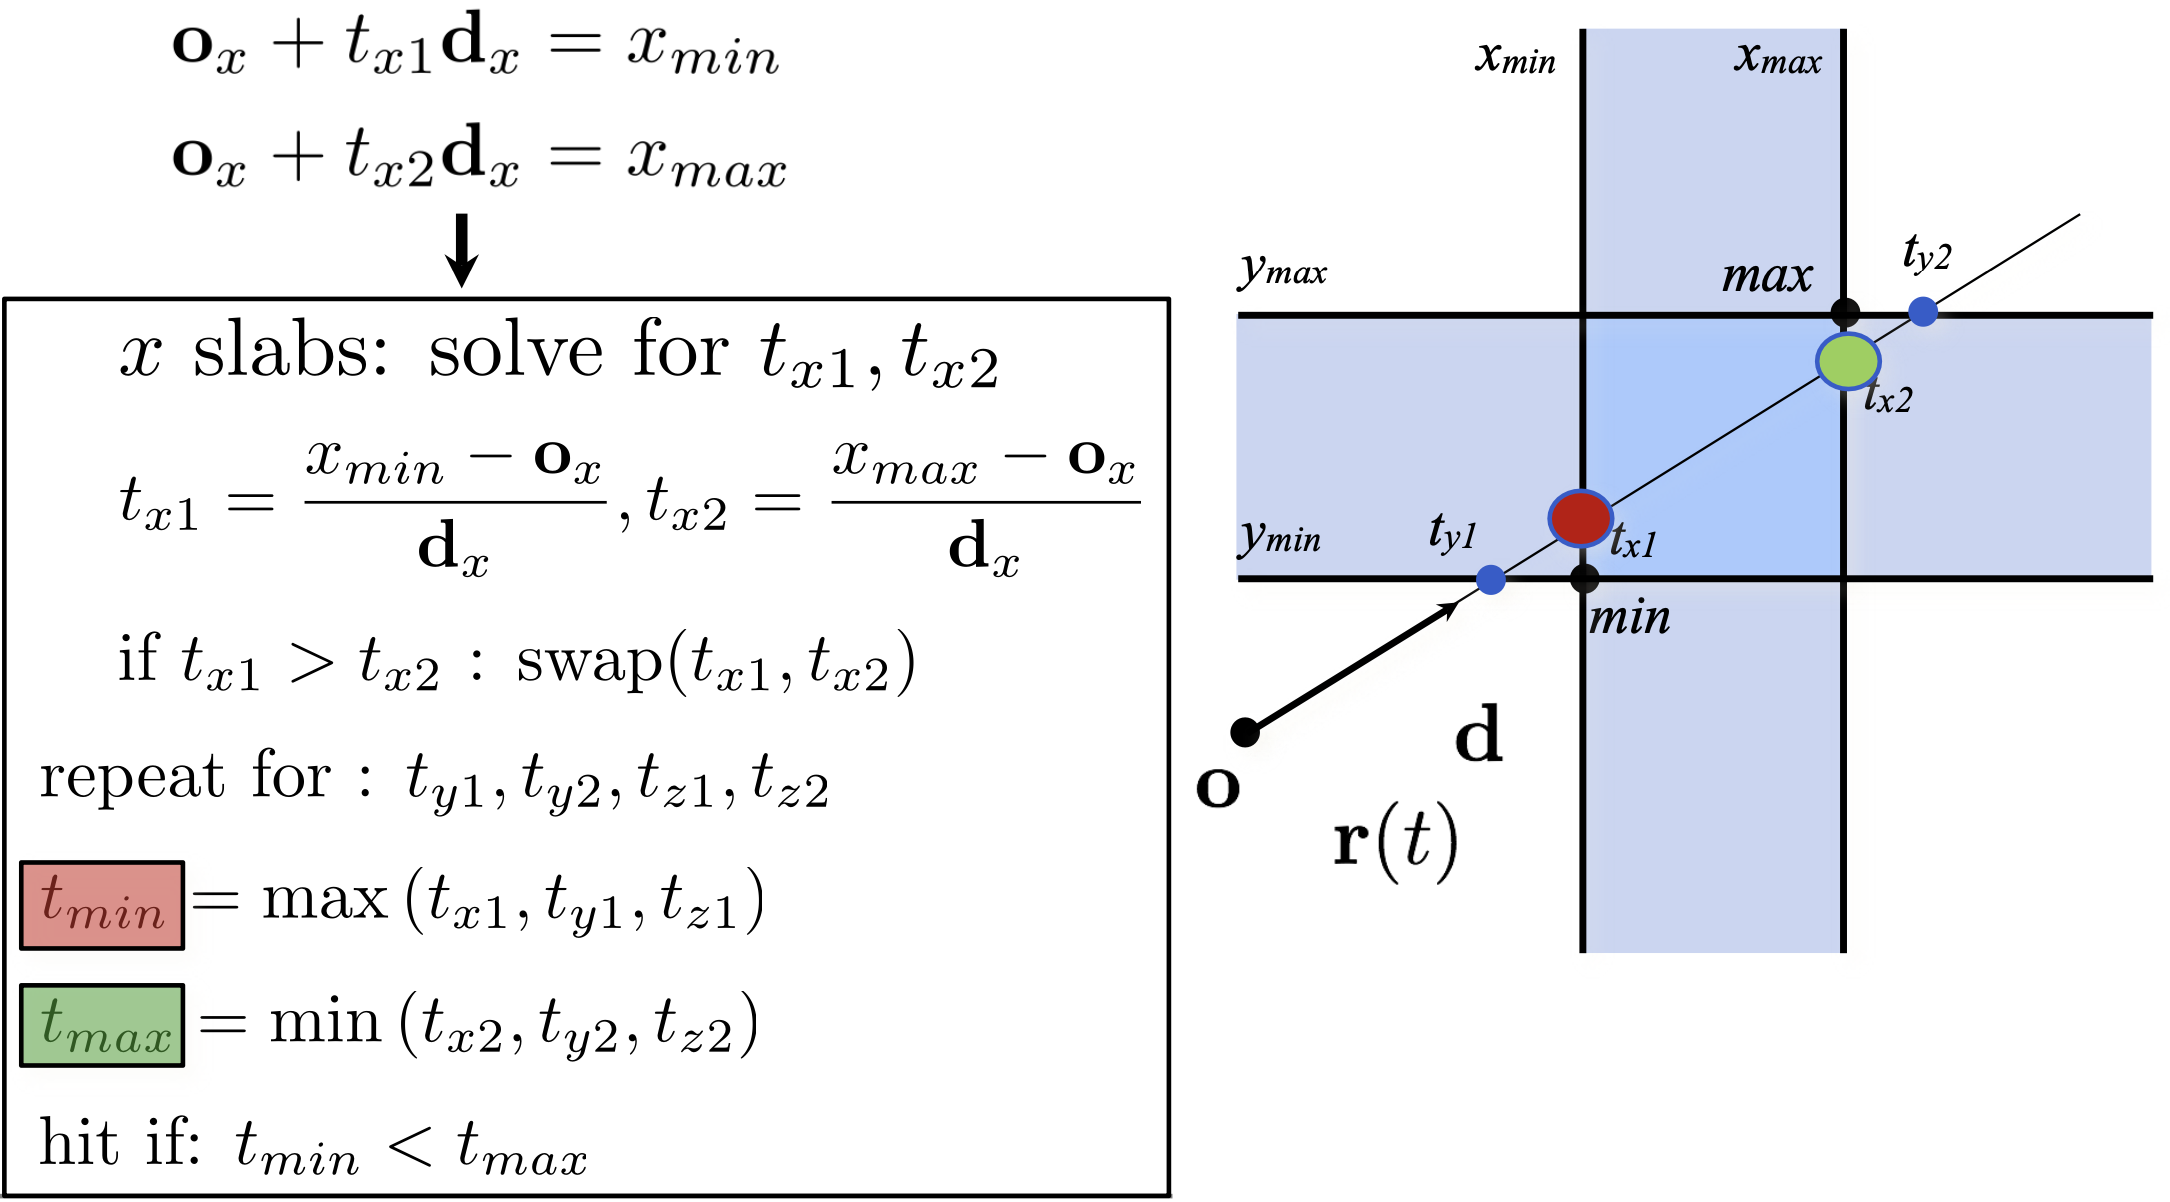
\includegraphics[width=\linewidth]{ray_aabb.png}
\end{center}

The main focus of the acceleration data structures is to decompose space into disjoint regions and store pointers to overlapping objects within each region. When rendering we then have to traverse through regions overlapping the ray and calculate only the intersections for objects in each region until a hit is found.


\subsection{Uniform Grids}

The most basic of these data structures are uniform grids. We first need to compute the bounding box and then apply a determined grid resolution (often $\sim 3 \root 3 \of n$). Then we insert objects into cells, prune empty cells and store references for each object in a cell.
\begin{center}
	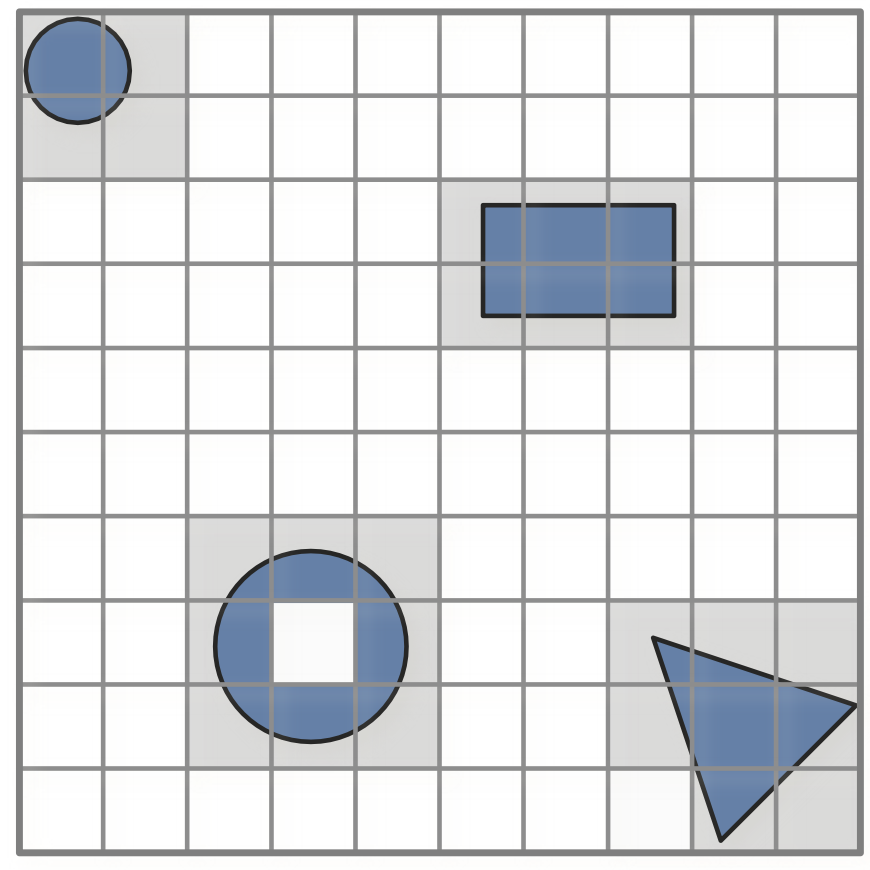
\includegraphics[width=0.6\linewidth]{uniform_grid.png}
\end{center}

During rendering, we incrementally rasterize the ray and compute the intersection with objects in each cell until we found a intersection. \medskip

This already gives a huge improvement over the brute fore approach and can be further refined by using hierarchical grids.


\subsection{Binary Space Partition}

There are different type of spacial hierarchies. They all follow the same divide-and-conquer approach. This again results in a lot fewer intersection tests.
\begin{center}
	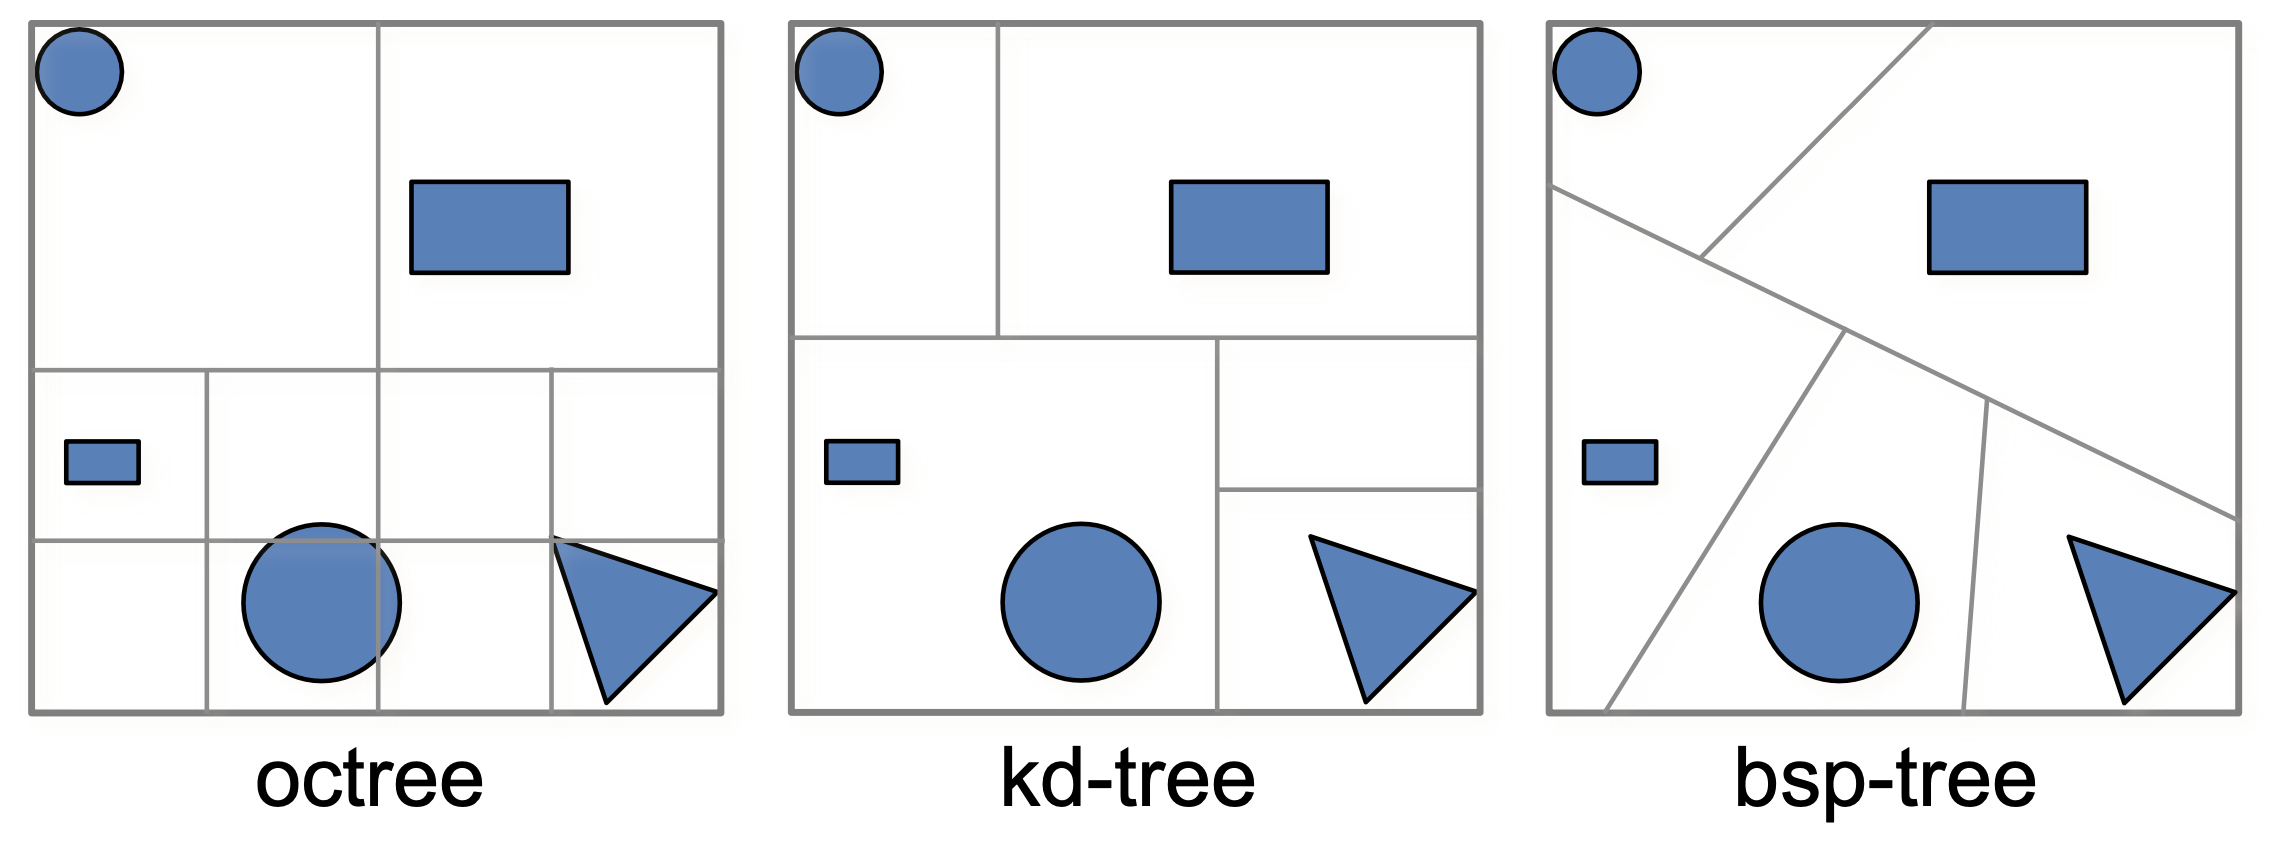
\includegraphics[width=\linewidth]{spatial_hierarchy.png}
\end{center}
From left to right we have increasing complexity but also more flexibility and fewer intersection tests.


\subsection{Bounding Volume Hierarchies}

Bounding volume hierarchies are an alternative divide-and-conquer method. It works by decomposing object into sets (overlapping) and bound them using simple volumes (spheres, axis-aligned bounding boxes, oriented bounding boxes). We can either apply top down or bottom up construction for this data structure.
\begin{center}
	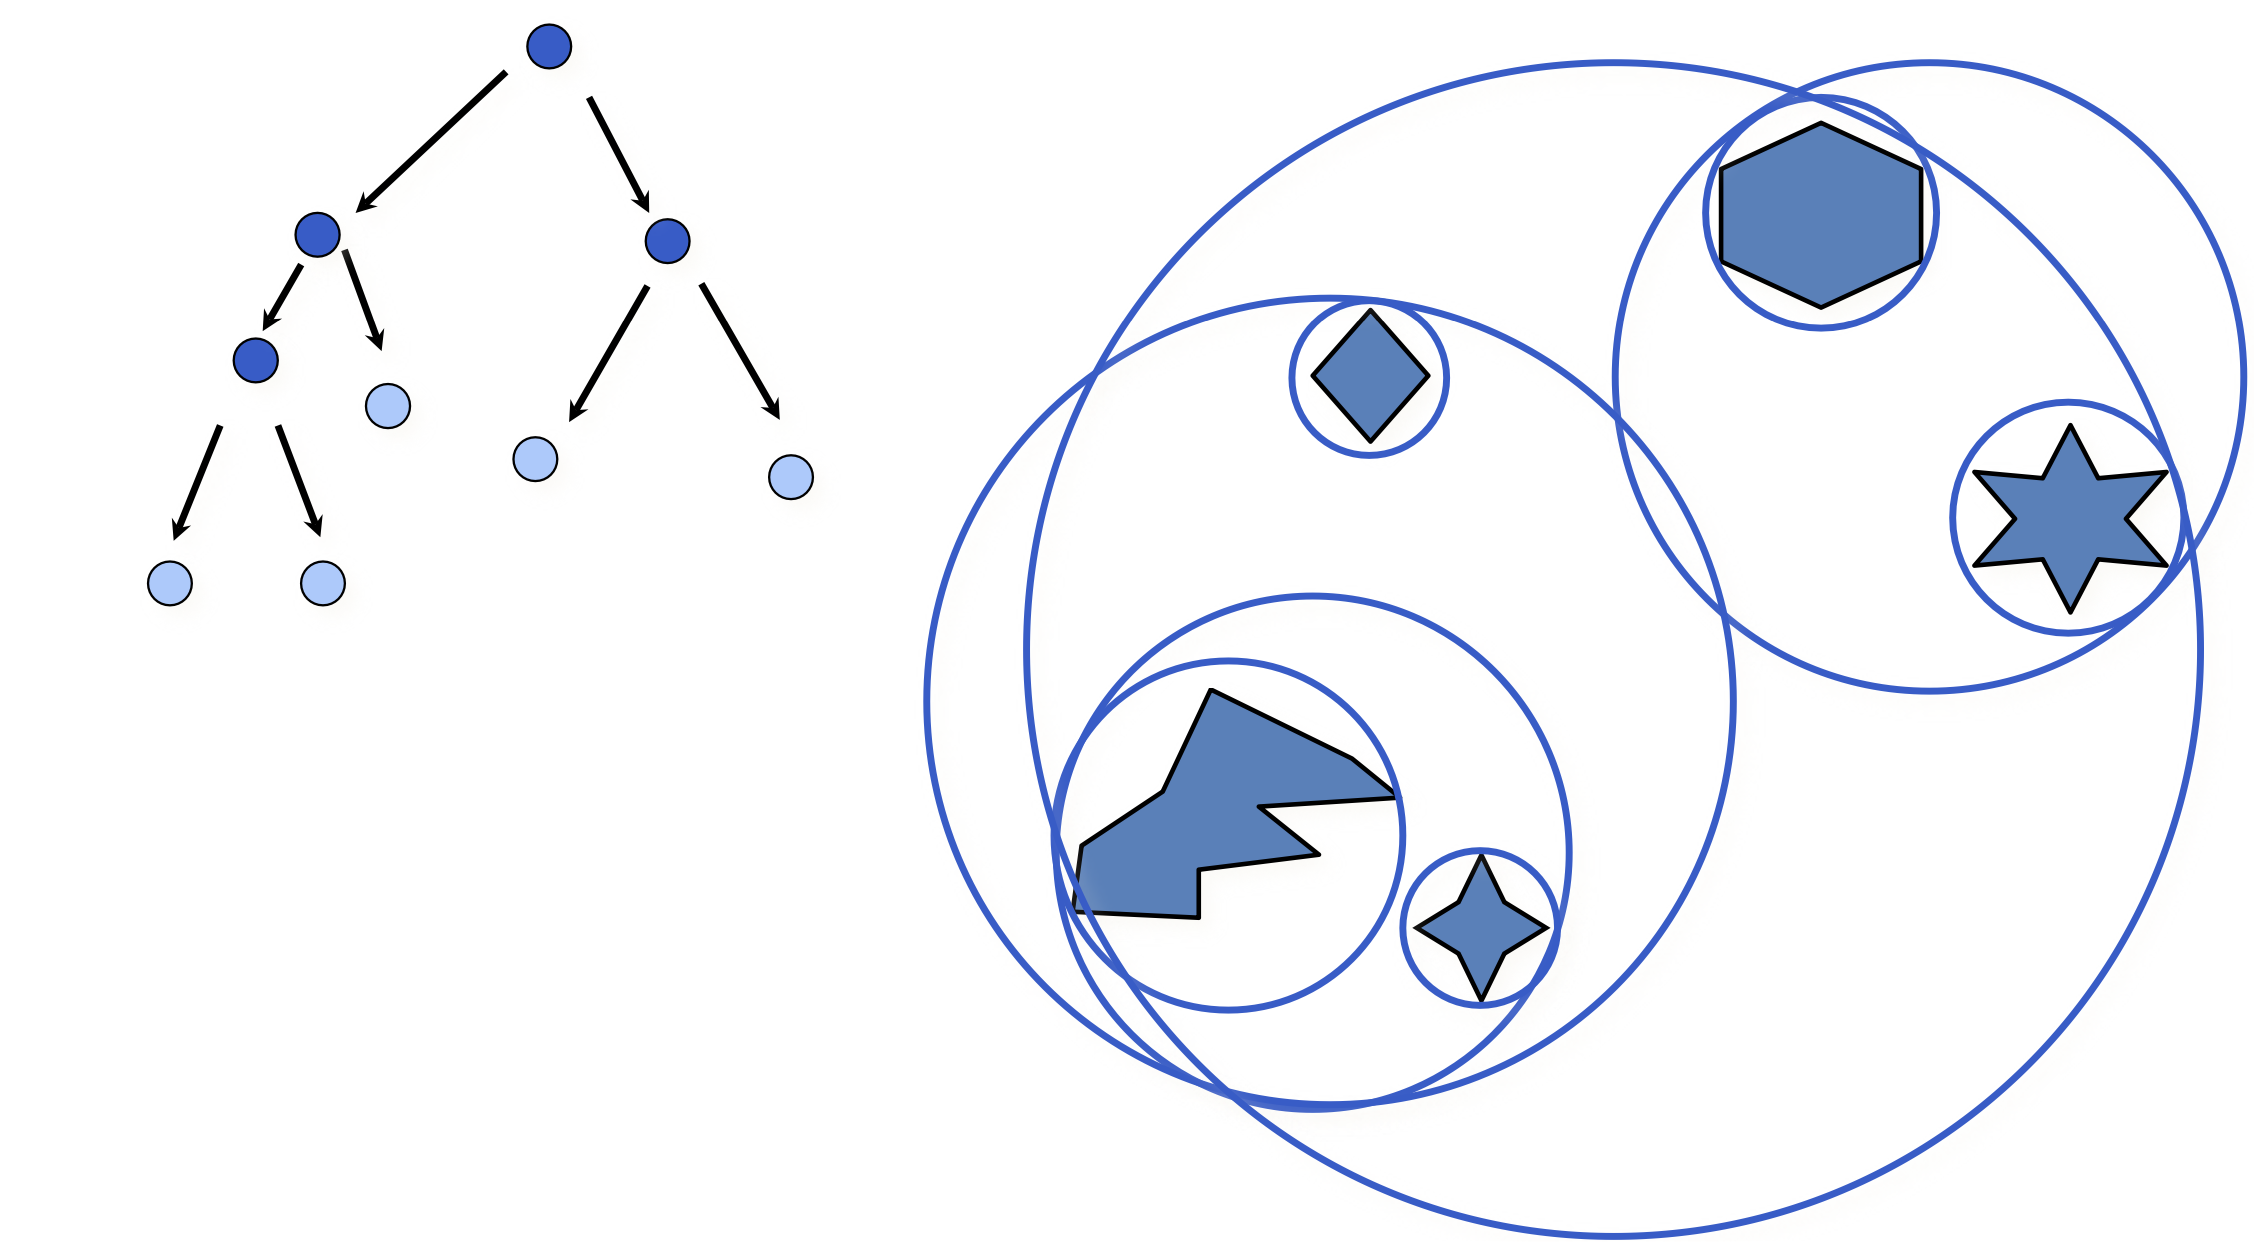
\includegraphics[width=\linewidth]{bounding_volume.png}
\end{center}